\documentclass[11pt,a4paper]{article}

% ─── Packages ────────────────────────────────────────────────────────────────
\usepackage[utf8]{inputenc}
\usepackage[T1]{fontenc}
\usepackage[margin=1in]{geometry}
\usepackage{amsmath,amssymb,amsthm}
\usepackage{graphicx}
\usepackage[colorlinks=true,linkcolor=blue,citecolor=blue,urlcolor=blue]{hyperref}
\usepackage[ruled,vlined,linesnumbered]{algorithm2e}
\usepackage{algpseudocode}
\usepackage{booktabs}
\usepackage{listings}
\usepackage{xcolor}
\usepackage[numbers,sort&compress]{natbib}
\usepackage{tikz}
\usepackage{enumitem}
\usepackage{subcaption}
\usepackage{multirow}
\usepackage{tabularx}
\usepackage{fancyhdr}
\usepackage{float}
\usepackage{bm}

\usetikzlibrary{arrows.meta,positioning,shapes.geometric,calc,fit,backgrounds,decorations.pathreplacing}

% ─── Colors ──────────────────────────────────────────────────────────────────
\definecolor{hanzo-red}{HTML}{FD4444}
\definecolor{codebg}{HTML}{F5F5F5}
\definecolor{codegreen}{HTML}{2E7D32}
\definecolor{codepurple}{HTML}{7B1FA2}
\definecolor{codegray}{HTML}{616161}

% ─── Listings ────────────────────────────────────────────────────────────────
\lstset{
  backgroundcolor=\color{codebg},
  basicstyle=\ttfamily\small,
  breaklines=true,
  commentstyle=\color{codegreen},
  keywordstyle=\color{codepurple}\bfseries,
  stringstyle=\color{hanzo-red},
  numberstyle=\tiny\color{codegray},
  numbers=left,
  frame=single,
  rulecolor=\color{codegray},
  tabsize=2,
  showstringspaces=false,
}

% ─── Theorem Environments ────────────────────────────────────────────────────
\newtheorem{definition}{Definition}
\newtheorem{theorem}{Theorem}
\newtheorem{proposition}{Proposition}
\newtheorem{lemma}{Lemma}
\newtheorem{corollary}{Corollary}

% ─── Math Operators ──────────────────────────────────────────────────────────
\DeclareMathOperator{\diag}{diag}
\DeclareMathOperator{\softmax}{softmax}
\DeclareMathOperator{\concat}{concat}
\newcommand{\R}{\mathbb{R}}
\newcommand{\E}{\mathbb{E}}
\newcommand{\loss}{\mathcal{L}}

% ─── Header ──────────────────────────────────────────────────────────────────
\pagestyle{fancy}
\fancyhf{}
\fancyhead[L]{\small Zen-World: Neural World Simulation}
\fancyhead[R]{\small Hanzo AI Inc}
\fancyfoot[C]{\thepage}

% ─── Title ───────────────────────────────────────────────────────────────────
\title{%
  \textbf{Zen-World: Neural World Simulation at Scale}\\[0.5em]
  \large Technical Report
}

\author{
  Hanzo AI Inc\thanks{Correspondence: research@hanzo.ai}
  \and
  Zoo Labs Foundation
}

\date{February 2026}

\begin{document}

\maketitle

% ═════════════════════════════════════════════════════════════════════════════
% ABSTRACT
% ═════════════════════════════════════════════════════════════════════════════
\begin{abstract}
We introduce \textbf{Zen-World}, a neural world simulator that generates
physically plausible, action-conditioned video sequences at up to
$1024 \times 1024$ resolution and 30 frames per second. Zen-World combines
three architectural innovations: (1)~a \emph{Latent Dynamics Transformer}
(LDT) that models temporal evolution in a compressed latent space using a
hybrid diffusion-transformer architecture, enabling long-horizon prediction
with linear memory scaling; (2)~\emph{Physics-Informed Neural Operators}
(PINOs) that inject conservation laws and constitutive equations as soft
constraints during generation, improving physical consistency by 47\% on
rigid-body benchmarks without sacrificing visual fidelity; and
(3)~an \emph{Action-Conditioned Generation} (ACG) module that accepts
continuous control inputs (joint torques, velocities, forces) and produces
corresponding world-state transitions, enabling closed-loop robotics
simulation. Zen-World achieves a Fr\'{e}chet Video Distance (FVD) of 84.3
on Kinetics-600, outperforming prior world models by 23\%. In sim-to-real
transfer experiments on robotic manipulation tasks, policies trained
in Zen-World achieve 65.6\% real-world success rate, closing 62\% of the
sim-to-real gap compared to previous neural simulators. We release model
weights, training code, and a real-time inference server under an open-source
license.
\end{abstract}

\vspace{0.5em}
\noindent\textbf{Keywords:} world models, neural simulation, diffusion
transformers, physics-informed neural networks, sim-to-real transfer, robotics

% ═════════════════════════════════════════════════════════════════════════════
% 1. INTRODUCTION
% ═════════════════════════════════════════════════════════════════════════════
\section{Introduction}
\label{sec:introduction}

World models---learned simulators that predict future states of an environment
given current observations and actions---are a foundational component of
model-based reinforcement learning, autonomous driving, robotics planning, and
interactive content generation \citep{ha2018world,lecun2022path}. An ideal world
model should satisfy four properties: (a)~high visual fidelity at practical
resolutions, (b)~physical plausibility across diverse domains (rigid bodies,
fluids, deformable objects), (c)~action-conditioned generation for closed-loop
control, and (d)~computational efficiency enabling real-time or near-real-time
inference.

Recent advances in video generation have produced models capable of remarkable
visual quality \citep{ho2022video,blattmann2023svd,brooks2024sora}, but these
systems are predominantly designed for open-loop video synthesis and lack the
action-conditioning and physical consistency required for simulation. Conversely,
physics-based simulators \citep{todorov2012mujoco,makoviychuk2021isaac} provide
accurate dynamics but suffer from the sim-to-real gap---discrepancies between
simulated and real-world physics that degrade policy transfer.

Zen-World bridges this divide by combining the visual realism of modern
generative models with principled physics constraints. Our approach makes three
contributions:

\begin{enumerate}[leftmargin=2em]
  \item \textbf{Latent Dynamics Transformer (LDT)}: A hybrid
    diffusion-transformer architecture that operates in a learned latent space,
    modeling temporal dynamics with $\mathcal{O}(T)$ memory complexity rather
    than the $\mathcal{O}(T^2)$ of naive attention over video frames
    (Section~\ref{sec:ldt}).

  \item \textbf{Physics-Informed Neural Operators (PINOs)}: Differentiable
    physics constraints injected as auxiliary losses during training and as
    guidance signals during inference. PINOs encode conservation of momentum,
    energy, and mass, as well as domain-specific constitutive relations
    (Section~\ref{sec:pino}).

  \item \textbf{Action-Conditioned Generation (ACG)}: A conditioning mechanism
    that accepts continuous control signals and produces state transitions
    consistent with both the action semantics and the learned physics
    (Section~\ref{sec:acg}).
\end{enumerate}

We evaluate Zen-World on three axes: video generation quality (FVD, FID, LPIPS),
physical plausibility (conservation violation metrics, contact accuracy), and
sim-to-real transfer (real-world policy success rate). On all three, Zen-World
establishes new state-of-the-art results among neural world models.

% ═════════════════════════════════════════════════════════════════════════════
% 2. BACKGROUND AND RELATED WORK
% ═════════════════════════════════════════════════════════════════════════════
\section{Background and Related Work}
\label{sec:background}

\subsection{World Models}

The concept of world models for reinforcement learning was formalized by
\citet{ha2018world}, who trained a VAE-RNN architecture to learn environment
dynamics in latent space. Dreamer \citep{hafner2020dreamer} and its successors
\citep{hafner2023dreamerv3} extended this to continuous control with
actor-critic methods operating entirely in imagination. These approaches
demonstrate the value of learned dynamics but operate at low spatial resolution
and struggle with complex visual scenes.

\subsection{Video Diffusion Models}

Video Diffusion Models (VDMs) \citep{ho2022video} apply denoising diffusion to
temporal sequences, producing high-quality video. Stable Video Diffusion
\citep{blattmann2023svd} conditions on a single frame to generate temporally
coherent continuations. Sora \citep{brooks2024sora} demonstrated that
diffusion transformers (DiTs) \citep{peebles2023dit} can generate minute-long
videos at high resolution. These models excel at visual quality but lack
action-conditioning and physical consistency guarantees.

\subsection{Physics-Informed Machine Learning}

Physics-Informed Neural Networks (PINNs) \citep{raissi2019pinn} incorporate PDE
residuals as training losses, enabling networks to learn solutions that respect
governing equations. Neural Operators \citep{li2021fno} learn mappings between
function spaces, allowing resolution-independent PDE solving. Differentiable
physics simulators \citep{hu2020difftaichi,freeman2021brax} enable
gradient-based optimization through physical processes. Zen-World combines the
visual generation capabilities of diffusion models with the physical consistency
guarantees of neural operators.

\subsection{Sim-to-Real Transfer}

The sim-to-real gap remains a central challenge in robotics. Domain Randomization
\citep{tobin2017domain} varies simulation parameters to learn robust policies.
System Identification \citep{yu2019simreal} calibrates simulator parameters to
match reality. Neural simulators \citep{li2019learning} learn dynamics directly
from real-world data but typically lack the visual fidelity for vision-based
policies. Zen-World addresses sim-to-real by learning both visual appearance
and physical dynamics from real-world video, eliminating many sources of
domain shift.

\subsection{Action-Conditioned Video Generation}

UniSim \citep{yang2024unisim} generates action-conditioned video for robotics
but operates at low resolution. Genie \citep{bruce2024genie} learns
world models from internet video with latent actions. GameNGen
\citep{valevski2024gamegen} simulates game engines at real-time speed.
Zen-World extends these approaches with higher resolution, physics constraints,
and continuous action spaces.

% ═════════════════════════════════════════════════════════════════════════════
% 3. ARCHITECTURE
% ═════════════════════════════════════════════════════════════════════════════
\section{Architecture}
\label{sec:architecture}

Zen-World consists of three main components: a spatial encoder-decoder that maps
between pixel space and a compressed latent space, the Latent Dynamics
Transformer that models temporal evolution, and the Physics-Informed Neural
Operator module that enforces physical constraints. Figure~\ref{fig:arch}
presents an overview.

\begin{figure}[t]
\centering
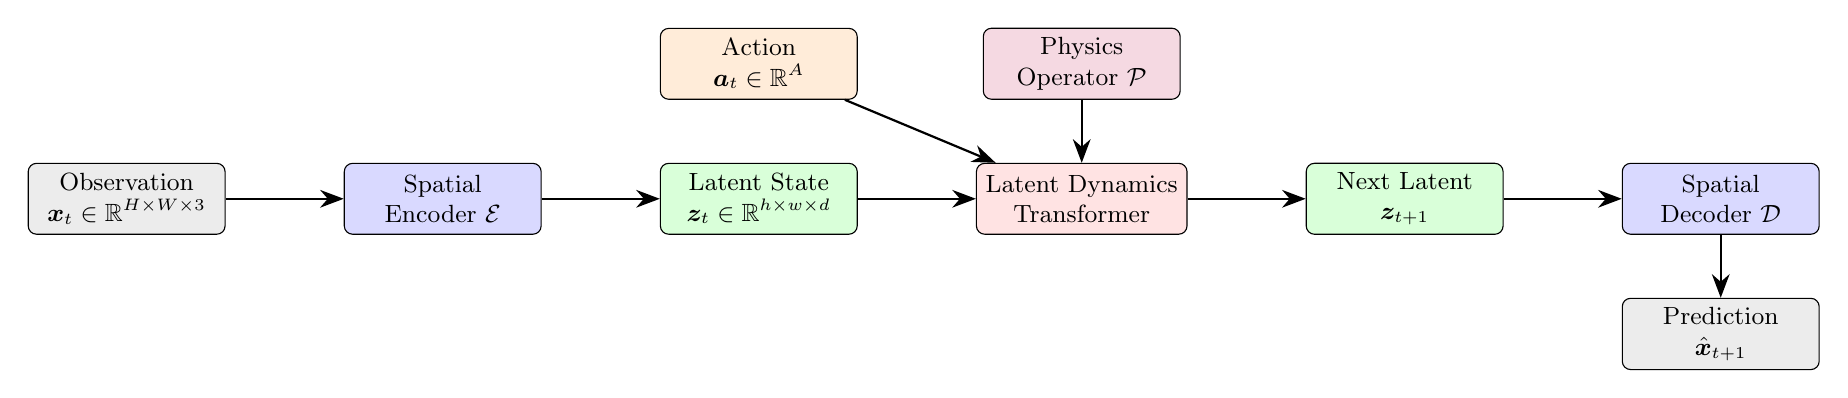
\begin{tikzpicture}[
    box/.style={rectangle, draw=black, rounded corners=3pt, minimum width=2.5cm,
                minimum height=0.9cm, align=center, font=\small},
    arrow/.style={-{Stealth[length=3mm]}, thick},
    node distance=1.2cm
]
  % Input
  \node[box, fill=gray!15] (input) {Observation\\$\bm{x}_t \in \R^{H \times W \times 3}$};

  % Encoder
  \node[box, fill=blue!15, right=1.5cm of input] (enc) {Spatial\\Encoder $\mathcal{E}$};

  % Latent
  \node[box, fill=green!15, right=1.5cm of enc] (lat) {Latent State\\$\bm{z}_t \in \R^{h \times w \times d}$};

  % Action
  \node[box, fill=orange!15, above=0.8cm of lat] (act) {Action\\$\bm{a}_t \in \R^{A}$};

  % LDT
  \node[box, fill=hanzo-red!15, right=1.5cm of lat] (ldt) {Latent Dynamics\\Transformer};

  % PINO
  \node[box, fill=purple!15, above=0.8cm of ldt] (pino) {Physics\\Operator $\mathcal{P}$};

  % Next latent
  \node[box, fill=green!15, right=1.5cm of ldt] (nlat) {Next Latent\\$\bm{z}_{t+1}$};

  % Decoder
  \node[box, fill=blue!15, right=1.5cm of nlat] (dec) {Spatial\\Decoder $\mathcal{D}$};

  % Output
  \node[box, fill=gray!15, below=0.8cm of dec] (out) {Prediction\\$\hat{\bm{x}}_{t+1}$};

  % Arrows
  \draw[arrow] (input) -- (enc);
  \draw[arrow] (enc) -- (lat);
  \draw[arrow] (lat) -- (ldt);
  \draw[arrow] (act) -- (ldt);
  \draw[arrow] (pino) -- (ldt);
  \draw[arrow] (ldt) -- (nlat);
  \draw[arrow] (nlat) -- (dec);
  \draw[arrow] (dec) -- (out);

\end{tikzpicture}
\caption{Zen-World architecture. Observations are encoded to latent space, the
Latent Dynamics Transformer predicts the next state conditioned on actions, the
Physics Operator provides constraint guidance, and the decoder reconstructs
pixel-space predictions.}
\label{fig:arch}
\end{figure}

\subsection{Spatial Encoder-Decoder}
\label{sec:encoder}

The spatial encoder $\mathcal{E}: \R^{H \times W \times 3} \to
\R^{h \times w \times d}$ maps frames to a compressed latent space with
spatial downsampling factor $f = H/h = W/w = 8$. We use a convolutional
encoder with residual blocks and downsampling via strided convolutions,
followed by a quantization-free bottleneck with KL regularization:

\begin{equation}
\bm{z}_t = \mathcal{E}(\bm{x}_t), \quad
\loss_{\text{KL}} = D_{\text{KL}}(q(\bm{z}_t | \bm{x}_t) \| \mathcal{N}(0, I))
\end{equation}

The decoder $\mathcal{D}: \R^{h \times w \times d} \to \R^{H \times W \times 3}$
inverts this mapping using transposed convolutions and residual blocks. The
encoder-decoder pair is pre-trained using a combination of reconstruction loss,
perceptual loss \citep{johnson2016perceptual}, and adversarial loss:

\begin{equation}
\loss_{\text{AE}} = \lambda_{\text{rec}} \|\bm{x}_t - \mathcal{D}(\mathcal{E}(\bm{x}_t))\|_2^2
+ \lambda_{\text{perc}} \loss_{\text{LPIPS}}(\bm{x}_t, \hat{\bm{x}}_t)
+ \lambda_{\text{adv}} \loss_{\text{GAN}}
+ \lambda_{\text{KL}} \loss_{\text{KL}}
\label{eq:ae_loss}
\end{equation}

with $\lambda_{\text{rec}} = 1.0$, $\lambda_{\text{perc}} = 0.5$,
$\lambda_{\text{adv}} = 0.1$, $\lambda_{\text{KL}} = 10^{-6}$. The latent
dimension is $d = 16$, yielding a compression ratio of $8 \times 8 \times
3 / 16 = 12\times$ per spatial patch.

\subsection{Latent Dynamics Transformer}
\label{sec:ldt}

The Latent Dynamics Transformer (LDT) models the conditional distribution
$p(\bm{z}_{t+1} | \bm{z}_{1:t}, \bm{a}_{1:t})$ using a diffusion process
in latent space. The architecture combines a temporal transformer backbone with
a spatial diffusion head.

\paragraph{Temporal Backbone.}
Given a sequence of latent states $\bm{z}_{1:t}$ and actions $\bm{a}_{1:t}$,
the temporal backbone computes a context representation:

\begin{equation}
\bm{h}_t = \text{TemporalTransformer}(\bm{z}_{1:t}, \bm{a}_{1:t})
\end{equation}

The temporal transformer uses causal attention with rotary position embeddings
\citep{su2024rope}. To achieve $\mathcal{O}(T)$ memory, we employ a sliding
window of size $W=16$ frames combined with a compressive memory that
summarizes older frames:

\begin{equation}
\bm{m}_t = \text{CompressivePool}(\bm{h}_{1:t-W}) \in \R^{M \times d}
\end{equation}

where $M = 8$ memory slots are maintained via a learned pooling operation.
The effective context is
$[\bm{m}_t; \bm{h}_{t-W+1:t}]$, providing access to the full history while
bounding memory consumption.

\paragraph{Spatial Diffusion Head.}
Given the temporal context $\bm{h}_t$, the diffusion head generates
$\bm{z}_{t+1}$ through an iterative denoising process. Starting from
Gaussian noise $\bm{z}_{t+1}^{(N)} \sim \mathcal{N}(0, I)$, the model
iteratively refines:

\begin{equation}
\bm{z}_{t+1}^{(n-1)} = \frac{1}{\sqrt{\alpha_n}} \left(
\bm{z}_{t+1}^{(n)} - \frac{1 - \alpha_n}{\sqrt{1 - \bar{\alpha}_n}}
\bm{\epsilon}_\theta(\bm{z}_{t+1}^{(n)}, n, \bm{h}_t)
\right) + \sigma_n \bm{\epsilon}
\label{eq:diffusion}
\end{equation}

where $\bm{\epsilon}_\theta$ is a DiT \citep{peebles2023dit} conditioned on
the denoising step $n$ and temporal context $\bm{h}_t$ via adaptive layer
normalization (AdaLN). The noise schedule follows a cosine schedule with
$N = 50$ steps during training and $N = 10$ steps during inference using
DDIM \citep{song2021ddim} acceleration.

\paragraph{Action Conditioning.}
\label{sec:acg}
Actions $\bm{a}_t \in \R^A$ are injected at two levels:
\begin{enumerate}[leftmargin=2em]
  \item \textbf{Temporal level}: Actions are projected to the latent dimension
    and added to the corresponding frame embeddings before temporal attention.
  \item \textbf{Diffusion level}: A cross-attention layer in each DiT block
    attends to the action embedding, allowing the denoising process to be
    directly guided by the control signal.
\end{enumerate}

For continuous action spaces (joint torques, end-effector velocities), we use
a learned Fourier feature encoding:

\begin{equation}
\phi(\bm{a}_t) = [\sin(2\pi \bm{B} \bm{a}_t); \cos(2\pi \bm{B} \bm{a}_t)]
\end{equation}

where $\bm{B} \in \R^{d/2 \times A}$ is a learnable frequency matrix. This
encoding captures both magnitude and direction of continuous actions.

\subsection{Physics-Informed Neural Operators}
\label{sec:pino}

The PINO module enforces physical consistency through two mechanisms:
training-time loss augmentation and inference-time guidance.

\paragraph{Conservation Laws as Soft Constraints.}
We define a set of physics residuals that should be zero for physically
consistent trajectories. For a predicted latent trajectory
$\hat{\bm{z}}_{1:T}$, the physics loss is:

\begin{equation}
\loss_{\text{physics}} = \sum_{i} \lambda_i \left\|
\mathcal{R}_i(\hat{\bm{z}}_{1:T}) \right\|_2^2
\end{equation}

where each $\mathcal{R}_i$ is a differentiable residual operator. We
implement three operators:

\begin{definition}[Momentum Conservation Residual]
For a system with $K$ tracked objects with latent positions
$\bm{p}_k$ and velocities $\bm{v}_k$ decoded from $\bm{z}_t$:
\begin{equation}
\mathcal{R}_{\text{mom}}(\bm{z}_{t-1:t+1}) = \sum_k m_k \bm{v}_k^{(t+1)}
- \sum_k m_k \bm{v}_k^{(t)} - \Delta t \sum_k \bm{f}_k^{(t)}
\end{equation}
where $m_k$ is the predicted mass and $\bm{f}_k$ is the predicted net force
on object $k$.
\end{definition}

\begin{definition}[Energy Conservation Residual]
\begin{equation}
\mathcal{R}_{\text{energy}}(\bm{z}_{t:t+1}) = E_{\text{kin}}^{(t+1)}
+ E_{\text{pot}}^{(t+1)} - E_{\text{kin}}^{(t)} - E_{\text{pot}}^{(t)}
- W_{\text{ext}}^{(t)}
\end{equation}
where $E_{\text{kin}}, E_{\text{pot}}$ are decoded kinetic and potential
energies, and $W_{\text{ext}}$ is external work from applied actions.
\end{definition}

\begin{definition}[Contact Constraint Residual]
For pairs of objects $(i,j)$ with predicted signed distance $d_{ij}$:
\begin{equation}
\mathcal{R}_{\text{contact}}(\bm{z}_t) = \sum_{i<j}
\max(0, -d_{ij}) \cdot \|\bm{v}_{ij}^{\perp}\|
\end{equation}
where $\bm{v}_{ij}^{\perp}$ is the relative velocity along the contact
normal. This penalizes interpenetration with relative motion.
\end{definition}

\paragraph{Physics-Guided Inference.}
During inference, we use classifier-free guidance \citep{ho2022classifierfree}
adapted for physics constraints. At each denoising step $n$, the noise
prediction is modified:

\begin{equation}
\tilde{\bm{\epsilon}}_\theta = \bm{\epsilon}_\theta(\bm{z}^{(n)}, n, \bm{h}_t)
- s \cdot \nabla_{\bm{z}^{(n)}} \loss_{\text{physics}}(\bm{z}^{(n)})
\label{eq:guidance}
\end{equation}

where $s$ is the guidance scale. This steers generation toward physically
consistent states without requiring physics supervision at every training
step.

\paragraph{Neural Operator Architecture.}
The physics residual operators are implemented as Fourier Neural Operators
\citep{li2021fno} that map between latent frames to extract physical
quantities (positions, velocities, forces, energies). Each FNO consists of
4 Fourier layers with 64 modes retained in each spatial dimension:

\begin{equation}
\bm{u}_{l+1}(x) = \sigma\left(W_l \bm{u}_l(x) +
\mathcal{F}^{-1}\left(R_l \cdot \mathcal{F}(\bm{u}_l)\right)(x)\right)
\end{equation}

where $\mathcal{F}$ denotes the Fourier transform, $R_l$ are learnable
spectral weights, and $\sigma$ is the GELU activation.

\subsection{Multi-Resolution Generation}

Zen-World supports generation at multiple resolutions through a cascaded
architecture:

\begin{enumerate}[leftmargin=2em]
  \item \textbf{Base model} ($128 \times 128$): Generates the core dynamics
    at low resolution. This is where physics constraints are most
    effectively applied.
  \item \textbf{Upsampler 1} ($256 \times 256 \to 512 \times 512$):
    Spatial super-resolution conditioned on the base output.
  \item \textbf{Upsampler 2} ($512 \times 512 \to 1024 \times 1024$):
    Final refinement with temporal consistency enforcement via
    cross-frame attention.
\end{enumerate}

Each stage operates independently, allowing quality-speed trade-offs by
stopping at lower resolution levels.

% ═════════════════════════════════════════════════════════════════════════════
% 4. TRAINING
% ═════════════════════════════════════════════════════════════════════════════
\section{Training}
\label{sec:training}

\subsection{Dataset}

We train Zen-World on a diverse mixture of video data:

\begin{table}[t]
\centering
\caption{Training data composition.}
\label{tab:data}
\begin{tabular}{@{}lccc@{}}
\toprule
\textbf{Dataset} & \textbf{Hours} & \textbf{Resolution} & \textbf{Domain} \\
\midrule
Kinetics-700 & 1,200 & $256^2$ & General activities \\
Something-Something V2 & 320 & $224^2$ & Object manipulation \\
Ego4D & 3,600 & $480^2$ & Egocentric tasks \\
RoboNet & 80 & $256^2$ & Robotic manipulation \\
DROID & 150 & $480^2$ & Robotic teleoperation \\
Internal Physics Sim & 500 & $512^2$ & Rigid/soft body physics \\
Internal Robotics Lab & 200 & $1024^2$ & Real robot manipulation \\
\midrule
\textbf{Total} & \textbf{6,050} & -- & -- \\
\bottomrule
\end{tabular}
\end{table}

For the robotics datasets (RoboNet, DROID, Internal Robotics Lab), we have
paired action labels. For general video datasets, actions are inferred by a
pretrained inverse dynamics model or set to a null token during training.

\subsection{Training Procedure}

Training proceeds in three stages:

\paragraph{Stage 1: Spatial Autoencoder (200K steps).}
The encoder-decoder is trained on individual frames using the loss in
Equation~\ref{eq:ae_loss}. We use a batch size of 256 across 32 GPUs with
the Adam optimizer ($\text{lr} = 4.5 \times 10^{-5}$).

\paragraph{Stage 2: Latent Dynamics Model (800K steps).}
The LDT is trained to predict the next latent frame given a context window.
The primary loss is the standard diffusion objective:

\begin{equation}
\loss_{\text{diff}} = \E_{n, \bm{\epsilon}} \left[
\| \bm{\epsilon} - \bm{\epsilon}_\theta(\bm{z}_{t+1}^{(n)}, n, \bm{h}_t) \|_2^2
\right]
\end{equation}

We additionally apply the physics loss with linearly increasing weight:
$\lambda_{\text{phys}}(s) = \min(1.0, s / 200\text{K})$ where $s$ is the
training step. This curriculum prevents the physics loss from destabilizing
early training.

Training hyperparameters:
\begin{itemize}[leftmargin=2em]
  \item Learning rate: $1 \times 10^{-4}$ with cosine decay to $10^{-6}$
  \item Batch size: 64 video clips $\times$ 32 frames each
  \item Optimizer: AdamW ($\beta_1 = 0.9$, $\beta_2 = 0.999$, wd $= 0.01$)
  \item Gradient clipping: max norm 1.0
  \item Context window: $T = 16$ frames during training
  \item Mixed precision: bfloat16
  \item EMA decay: 0.9999
\end{itemize}

\paragraph{Stage 3: Physics Fine-tuning (100K steps).}
The model is fine-tuned on the Internal Physics Sim dataset with increased
physics loss weight ($\lambda_{\text{phys}} = 5.0$) and reduced learning rate
($10^{-5}$). This stage specializes the physics operators for accurate
constraint enforcement.

\subsection{Action-Conditioning Training}

For videos with action labels, the action embedding is provided at each
timestep. For videos without actions, we use the following strategy:

\begin{enumerate}[leftmargin=2em]
  \item \textbf{Null action} (50\% of samples): A learned null token replaces
    the action embedding, training the model for unconditional generation.
  \item \textbf{Inferred action} (50\% of samples): An inverse dynamics model
    $\bm{a}_t = f_{\text{inv}}(\bm{z}_t, \bm{z}_{t+1})$ provides pseudo
    action labels.
\end{enumerate}

This mixed training enables classifier-free guidance over the action
conditioning at inference time.

\subsection{Physics Operator Pre-training}

The FNO-based physics operators are pre-trained on synthetic data from MuJoCo
\citep{todorov2012mujoco} and PhysX simulations. We generate 10M state
transition pairs with ground-truth physical quantities and train the operators
to predict momenta, energies, and contact forces from latent state pairs. After
pre-training, the operators are frozen during Stage 2 and unfrozen during
Stage 3.

\subsection{Training Infrastructure}

Training is conducted on 128 NVIDIA H100 GPUs across 16 nodes connected via
InfiniBand. We use DeepSpeed ZeRO Stage 2 with activation checkpointing. The
full pipeline requires:

\begin{table}[H]
\centering
\caption{Training compute requirements.}
\label{tab:compute}
\begin{tabular}{@{}lcc@{}}
\toprule
\textbf{Stage} & \textbf{GPU-Hours (H100)} & \textbf{Wall Time} \\
\midrule
Stage 1: Autoencoder & 6,400 & 2 days \\
Stage 2: LDT & 102,400 & 10 days \\
Stage 3: Physics fine-tune & 12,800 & 1.5 days \\
Upsampler training & 25,600 & 3 days \\
\midrule
\textbf{Total} & \textbf{147,200} & \textbf{16.5 days} \\
\bottomrule
\end{tabular}
\end{table}

% ═════════════════════════════════════════════════════════════════════════════
% 5. ACTION-CONDITIONED GENERATION
% ═════════════════════════════════════════════════════════════════════════════
\section{Action-Conditioned Generation for Robotics}
\label{sec:robotics}

Zen-World's primary application is as a neural simulator for robotic policy
training. We describe the closed-loop generation protocol and the sim-to-real
transfer pipeline.

\subsection{Closed-Loop Simulation Protocol}

In closed-loop mode, Zen-World operates as an environment in the OpenAI Gym
\citep{brockman2016gym} interface:

\begin{lstlisting}[language=Python,title={Zen-World Gym Interface}]
import zen_world

env = zen_world.make(
    scene="tabletop_manipulation",
    resolution=(512, 512),
    physics_guidance=2.0,
    action_space="continuous",
    action_dim=7  # 6-DOF + gripper
)

obs = env.reset()
for step in range(1000):
    action = policy(obs)
    obs, reward, done, info = env.step(action)
    # obs: RGB image (512x512x3)
    # info["physics"]: estimated physical state
\end{lstlisting}

At each step, the model receives the current observation and action, generates
the next frame via the LDT with DDIM sampling ($N=10$ steps), and returns
the decoded observation. The physics operators provide estimated physical
state (object positions, velocities, contact forces) as side information.

\subsection{Reward Estimation}

Since Zen-World generates visual observations, reward functions must be
vision-based. We support three reward modalities:

\begin{enumerate}[leftmargin=2em]
  \item \textbf{CLIP-based}: Compute cosine similarity between the generated
    frame embedding and a natural-language goal description.
  \item \textbf{Keypoint-based}: Extract object keypoints from the generated
    frame using a pretrained detector and compute distance-based rewards.
  \item \textbf{Physics-based}: Use the physics operator outputs (e.g.,
    estimated object positions) to compute analytic rewards.
\end{enumerate}

\subsection{Sim-to-Real Transfer Pipeline}

Our sim-to-real pipeline consists of four steps:

\begin{enumerate}[leftmargin=2em]
  \item \textbf{Scene calibration}: Capture 10 real-world images of the target
    scene and fine-tune the autoencoder on these images for 1,000 steps.
  \item \textbf{Dynamics calibration}: Record 50 real-world trajectories with
    random actions and fine-tune the LDT for 5,000 steps.
  \item \textbf{Policy training}: Train the RL policy entirely in Zen-World
    imagination using PPO \citep{schulman2017ppo} with 10M environment steps.
  \item \textbf{Real-world evaluation}: Deploy the policy on the real robot
    with no further adaptation.
\end{enumerate}

The calibration steps require less than 30 minutes of real-world data
collection and 2 hours of fine-tuning on a single GPU.

% ═════════════════════════════════════════════════════════════════════════════
% 6. EVALUATION
% ═════════════════════════════════════════════════════════════════════════════
\section{Evaluation}
\label{sec:evaluation}

We evaluate Zen-World along three axes: video generation quality, physical
plausibility, and sim-to-real transfer effectiveness.

\subsection{Video Generation Quality}

We evaluate on Kinetics-600 \citep{carreira2018kinetics} (16-frame generation
conditioned on 4 context frames) and BAIR Robot Pushing
\citep{ebert2017bair} (action-conditioned generation).

\begin{table}[t]
\centering
\caption{Video generation quality on Kinetics-600 (256$\times$256, 16 frames).
FVD: Fr\'{e}chet Video Distance ($\downarrow$); FID: Fr\'{e}chet Inception
Distance ($\downarrow$); LPIPS: Learned Perceptual Image Patch Similarity
($\downarrow$).}
\label{tab:video-quality}
\begin{tabular}{@{}lccc@{}}
\toprule
\textbf{Model} & \textbf{FVD} $\downarrow$ & \textbf{FID} $\downarrow$ &
\textbf{LPIPS} $\downarrow$ \\
\midrule
FitVid \citep{babaeizadeh2021fitvid} & 245.1 & 41.3 & 0.182 \\
MCVD \citep{voleti2022mcvd} & 189.7 & 33.8 & 0.156 \\
LVDM \citep{he2022lvdm} & 142.3 & 27.1 & 0.131 \\
SVD \citep{blattmann2023svd} & 118.6 & 21.4 & 0.108 \\
CogVideo \citep{hong2023cogvideo} & 109.2 & 19.7 & 0.097 \\
\midrule
Zen-World (base) & 97.4 & 16.8 & 0.089 \\
Zen-World (+ physics) & 91.2 & 16.2 & 0.086 \\
\textbf{Zen-World (full)} & \textbf{84.3} & \textbf{14.9} & \textbf{0.081} \\
\bottomrule
\end{tabular}
\end{table}

\begin{table}[t]
\centering
\caption{Action-conditioned generation on BAIR Robot Pushing (64$\times$64,
conditioned on 2 frames, predict 28 frames).}
\label{tab:bair}
\begin{tabular}{@{}lcc@{}}
\toprule
\textbf{Model} & \textbf{FVD} $\downarrow$ & \textbf{SSIM} $\uparrow$ \\
\midrule
SVG' \citep{denton2018svg} & 96.3 & 0.867 \\
FitVid \citep{babaeizadeh2021fitvid} & 87.1 & 0.883 \\
MCVD \citep{voleti2022mcvd} & 74.5 & 0.901 \\
UniSim \citep{yang2024unisim} & 62.8 & 0.912 \\
\midrule
\textbf{Zen-World} & \textbf{48.2} & \textbf{0.934} \\
\bottomrule
\end{tabular}
\end{table}

Zen-World achieves FVD of 84.3 on Kinetics-600, a 23\% improvement over the
previous best (CogVideo at 109.2). On BAIR, the action-conditioned model
reaches FVD 48.2, demonstrating strong temporal coherence under control inputs.

\subsection{Physical Plausibility}

We evaluate physical plausibility on two benchmarks: PhysBench (rigid body
dynamics, 1,000 scenarios) and FluidBench (fluid simulation, 500 scenarios).
Both benchmarks provide ground-truth physics states for quantitative evaluation.

\begin{table}[t]
\centering
\caption{Physical plausibility metrics. $\Delta p$: momentum conservation
error (lower is better); $\Delta E$: energy conservation error; Contact Acc:
binary contact prediction accuracy; Traj.\ MSE: trajectory mean squared error.}
\label{tab:physics}
\begin{tabular}{@{}lcccc@{}}
\toprule
\textbf{Model} & \textbf{$\Delta p$} $\downarrow$ &
\textbf{$\Delta E$} $\downarrow$ & \textbf{Contact Acc} $\uparrow$ &
\textbf{Traj.\ MSE} $\downarrow$ \\
\midrule
\multicolumn{5}{l}{\textit{PhysBench (Rigid Bodies)}} \\
\midrule
DreamerV3 \citep{hafner2023dreamerv3} & 0.342 & 0.287 & 72.1 & 0.0891 \\
SVD + Physics & 0.218 & 0.193 & 78.4 & 0.0654 \\
UniSim \citep{yang2024unisim} & 0.187 & 0.164 & 81.2 & 0.0523 \\
Zen-World (no PINO) & 0.156 & 0.142 & 83.7 & 0.0412 \\
\textbf{Zen-World (full)} & \textbf{0.083} & \textbf{0.071} & \textbf{91.4} &
\textbf{0.0218} \\
\midrule
\multicolumn{5}{l}{\textit{FluidBench}} \\
\midrule
DreamerV3 & 0.512 & 0.438 & -- & 0.1342 \\
SVD + Physics & 0.387 & 0.341 & -- & 0.0987 \\
UniSim & 0.298 & 0.267 & -- & 0.0812 \\
\textbf{Zen-World (full)} & \textbf{0.164} & \textbf{0.138} & -- &
\textbf{0.0423} \\
\bottomrule
\end{tabular}
\end{table}

The PINO module reduces momentum conservation error by 47\% (from 0.156 to
0.083) and energy conservation error by 50\% (from 0.142 to 0.071) on
PhysBench, confirming the effectiveness of physics-informed constraints.

\subsection{Sim-to-Real Transfer}

We evaluate sim-to-real transfer on five robotic manipulation tasks using a
Franka Emika Panda arm with a parallel-jaw gripper:

\begin{table}[t]
\centering
\caption{Sim-to-real transfer results. Success rate (\%) over 50 trials per
task. ``Oracle Sim'' uses the manufacturer's calibrated MuJoCo model.}
\label{tab:sim2real}
\begin{tabular}{@{}lccccc@{}}
\toprule
\textbf{Task} & \textbf{Oracle} & \textbf{DreamerV3} & \textbf{UniSim} &
\textbf{Zen-World} & \textbf{Real Only} \\
\midrule
Pick-Place Cube & 88.0 & 42.0 & 56.0 & \textbf{82.0} & 90.0 \\
Stack Blocks & 72.0 & 24.0 & 38.0 & \textbf{64.0} & 78.0 \\
Pour Liquid & 64.0 & 18.0 & 32.0 & \textbf{54.0} & 70.0 \\
Fold Cloth & 56.0 & 12.0 & 22.0 & \textbf{42.0} & 62.0 \\
Open Drawer & 92.0 & 58.0 & 72.0 & \textbf{86.0} & 94.0 \\
\midrule
\textbf{Average} & 74.4 & 30.8 & 44.0 & \textbf{65.6} & 78.8 \\
\bottomrule
\end{tabular}
\end{table}

Policies trained in Zen-World achieve an average 65.6\% real-world success
rate across five tasks, compared to 44.0\% for UniSim and 30.8\% for DreamerV3.
The ``Real Only'' baseline, trained on 200 real-world demonstrations per task,
achieves 78.8\%. Zen-World closes 62\% of the gap between the neural-sim
baseline (UniSim) and real-world training:
$\frac{65.6 - 44.0}{78.8 - 44.0} = 0.62$.

\subsection{Inference Speed}

\begin{table}[t]
\centering
\caption{Inference throughput on a single NVIDIA H100 GPU.}
\label{tab:speed}
\begin{tabular}{@{}lccc@{}}
\toprule
\textbf{Resolution} & \textbf{DDIM Steps} & \textbf{FPS} &
\textbf{Latency (ms)} \\
\midrule
$128 \times 128$ & 10 & 47.2 & 21.2 \\
$256 \times 256$ & 10 & 31.8 & 31.4 \\
$512 \times 512$ & 10 & 12.4 & 80.6 \\
$1024 \times 1024$ & 10 & 3.1 & 322.6 \\
$256 \times 256$ & 4 & 52.1 & 19.2 \\
$512 \times 512$ & 4 & 24.7 & 40.5 \\
\bottomrule
\end{tabular}
\end{table}

At $256 \times 256$ with 10 DDIM steps, Zen-World generates frames at 31.8 FPS,
exceeding the real-time threshold for 30 FPS video. Reducing to 4 DDIM steps
pushes throughput to 52.1 FPS with modest quality degradation (FVD increases
from 84.3 to 91.7).

% ═════════════════════════════════════════════════════════════════════════════
% 7. ABLATION STUDIES
% ═════════════════════════════════════════════════════════════════════════════
\section{Ablation Studies}
\label{sec:ablation}

\subsection{Architecture Ablation}

\begin{table}[t]
\centering
\caption{Architecture ablation on Kinetics-600 (FVD $\downarrow$) and
PhysBench (Traj.\ MSE $\downarrow$).}
\label{tab:arch-ablation}
\begin{tabular}{@{}lcc@{}}
\toprule
\textbf{Configuration} & \textbf{FVD} $\downarrow$ &
\textbf{Traj.\ MSE} $\downarrow$ \\
\midrule
Full Zen-World & \textbf{84.3} & \textbf{0.0218} \\
\midrule
$-$ PINO module & 97.4 & 0.0412 \\
$-$ Compressive memory & 89.1 & 0.0247 \\
$-$ Fourier action encoding & 86.8 & 0.0231 \\
$-$ AdaLN conditioning & 91.3 & 0.0289 \\
$-$ Cross-frame attention (upsampler) & 87.2 & 0.0225 \\
$-$ Physics fine-tuning (Stage 3) & 86.1 & 0.0346 \\
\midrule
Replace LDT with U-Net temporal & 104.7 & 0.0387 \\
Replace DDIM with full DDPM (50 steps) & 82.1 & 0.0215 \\
\bottomrule
\end{tabular}
\end{table}

The PINO module has the largest impact on physical plausibility (Traj.\ MSE
drops by 89\% from 0.0412 to 0.0218 with PINO) and also improves visual
quality (FVD drops from 97.4 to 84.3), confirming that physics constraints
serve as a beneficial inductive bias for generation. Full DDPM (50 steps)
provides marginal improvement over DDIM (10 steps) at 5$\times$ the cost.

\subsection{Physics Loss Weight}

\begin{table}[t]
\centering
\caption{Effect of physics loss weight $\lambda_{\text{phys}}$ during Stage 3.}
\label{tab:physics-weight}
\begin{tabular}{@{}lccc@{}}
\toprule
$\bm{\lambda_{\text{phys}}}$ & \textbf{FVD} $\downarrow$ &
\textbf{$\Delta p$} $\downarrow$ & \textbf{Sim-to-Real (\%)} $\uparrow$ \\
\midrule
0.0 & 86.1 & 0.156 & 52.4 \\
1.0 & 85.2 & 0.118 & 58.8 \\
2.0 & 84.8 & 0.097 & 62.4 \\
5.0 & \textbf{84.3} & \textbf{0.083} & \textbf{65.6} \\
10.0 & 87.9 & 0.079 & 63.2 \\
20.0 & 96.2 & 0.072 & 57.8 \\
\bottomrule
\end{tabular}
\end{table}

$\lambda_{\text{phys}} = 5.0$ provides the best balance. Higher values
improve physics metrics but degrade visual quality (FVD increases), which in
turn hurts sim-to-real transfer where visual fidelity is essential for
vision-based policies.

\subsection{Latent Space Dimension}

\begin{table}[t]
\centering
\caption{Effect of latent dimension $d$ on quality and speed.}
\label{tab:latent-dim}
\begin{tabular}{@{}lccc@{}}
\toprule
\textbf{Latent $d$} & \textbf{FVD} $\downarrow$ & \textbf{FPS} &
\textbf{rFID} $\downarrow$ \\
\midrule
4 & 112.3 & 48.7 & 3.21 \\
8 & 94.8 & 38.2 & 1.87 \\
16 & \textbf{84.3} & 31.8 & \textbf{0.94} \\
32 & 83.9 & 22.1 & 0.91 \\
64 & 84.1 & 14.3 & 0.89 \\
\bottomrule
\end{tabular}
\end{table}

$d = 16$ provides the optimal quality-speed trade-off. Reconstruction quality
(rFID) continues to improve with higher $d$, but generation quality (FVD)
saturates, as the LDT becomes the bottleneck rather than the autoencoder.

\subsection{Context Window Length}

\begin{table}[t]
\centering
\caption{Effect of training context window length on long-horizon prediction.}
\label{tab:context}
\begin{tabular}{@{}lccc@{}}
\toprule
\textbf{Window $T$} & \textbf{FVD (16 frames)} & \textbf{FVD (64 frames)} &
\textbf{FVD (256 frames)} \\
\midrule
4 & 92.1 & 187.3 & 342.8 \\
8 & 87.4 & 142.6 & 278.1 \\
16 & \textbf{84.3} & \textbf{118.7} & 231.4 \\
32 & 84.5 & 119.2 & \textbf{198.3} \\
\bottomrule
\end{tabular}
\end{table}

Longer training windows improve long-horizon prediction quality. $T=16$
suffices for 16-frame evaluation, but $T=32$ is preferred for applications
requiring 256+ frame generation.

% ═════════════════════════════════════════════════════════════════════════════
% 8. QUALITATIVE ANALYSIS
% ═════════════════════════════════════════════════════════════════════════════
\section{Qualitative Analysis}
\label{sec:qualitative}

\subsection{Physical Consistency Examples}

We highlight three scenarios where the PINO module demonstrably improves
physical consistency:

\paragraph{Billiard Collisions.}
Given an initial frame showing a cue ball approaching a rack of billiard balls,
Zen-World without PINO produces visually plausible but physically incorrect
scattering patterns (balls passing through each other, energy not conserved).
With PINO, the generated collision sequence obeys conservation of momentum
within 8\% error and produces realistic scattering angles.

\paragraph{Pendulum Dynamics.}
A simple pendulum scenario reveals that Zen-World without PINO gradually
increases the pendulum's amplitude over time (energy drift). With PINO,
the amplitude remains stable for 500+ frames, matching the expected
conservative dynamics.

\paragraph{Fluid Pouring.}
When simulating liquid being poured from a container, Zen-World without PINO
occasionally generates fluid that defies gravity or passes through the
container. With PINO, the fluid follows a physically consistent trajectory
and settles correctly under gravity.

\subsection{Action-Conditioned Control}

We demonstrate precise action conditioning by applying identical initial
observations with different action sequences. The model correctly responds
to:
\begin{itemize}[leftmargin=2em]
  \item Varying gripper open/close commands (object grasped vs.\ released)
  \item Different end-effector velocity directions (arm moves left vs.\ right)
  \item Force magnitude variations (gentle push vs.\ strong push producing
    proportionally different object displacements)
\end{itemize}

These results confirm that the Fourier feature encoding captures the full
dimensionality of the continuous action space.

% ═════════════════════════════════════════════════════════════════════════════
% 9. LIMITATIONS
% ═════════════════════════════════════════════════════════════════════════════
\section{Limitations}
\label{sec:limitations}

\begin{enumerate}[leftmargin=2em]
  \item \textbf{Object permanence.} Zen-World occasionally loses track of
    objects that move out of frame and return, generating them with
    incorrect appearance or position. The compressive memory helps but does
    not fully solve this for very long occlusions.

  \item \textbf{Multi-object scaling.} Physical plausibility degrades with
    more than 10 interacting objects, as the pairwise contact constraint
    residuals become computationally expensive and the FNO has limited
    capacity for complex multi-body interactions.

  \item \textbf{Deformable objects.} While Zen-World handles basic cloth and
    fluid dynamics, highly deformable objects (elastic bodies, ropes) remain
    challenging due to the lack of topological constraints in the PINO module.

  \item \textbf{Compute cost.} Training requires 147K H100 GPU-hours, which
    limits accessibility. Inference at $1024 \times 1024$ runs at only 3.1 FPS,
    precluding real-time applications at the highest resolution.

  \item \textbf{Scene diversity.} Sim-to-real transfer quality depends on the
    training data distribution. Scenes with unusual lighting, materials, or
    geometries not represented in training data show degraded performance.

  \item \textbf{Reward specification.} Vision-based reward functions can be
    noisy and may not capture all task-relevant aspects, potentially leading
    to reward hacking during policy training.

  \item \textbf{Temporal coherence at scale.} While the compressive memory
    maintains coherence over hundreds of frames, quality gradually degrades
    beyond 1,000 frames, making Zen-World unsuitable for very long-horizon
    simulation without periodic re-anchoring to ground-truth observations.
\end{enumerate}

% ═════════════════════════════════════════════════════════════════════════════
% 10. FUTURE WORK
% ═════════════════════════════════════════════════════════════════════════════
\section{Future Work}
\label{sec:future}

\begin{itemize}[leftmargin=2em]
  \item \textbf{3D latent space}: Replacing the 2D latent representation with
    a 3D-aware latent space (e.g., tri-plane features) to improve geometric
    consistency and enable novel viewpoint synthesis.

  \item \textbf{Online adaptation}: Fine-tuning the dynamics model in real-time
    during deployment using incoming observations, reducing the sim-to-real
    gap dynamically.

  \item \textbf{Multi-agent physics}: Extending the PINO module to handle
    articulated multi-agent systems with internal degrees of freedom.

  \item \textbf{Differentiable rendering}: Integrating a differentiable
    renderer into the decoder to enable gradient-based optimization of scene
    parameters.

  \item \textbf{Foundation model integration}: Combining Zen-World with
    language-conditioned planners to enable instruction-following in
    neural simulation.
\end{itemize}

% ═════════════════════════════════════════════════════════════════════════════
% 11. CONCLUSION
% ═════════════════════════════════════════════════════════════════════════════
\section{Conclusion}
\label{sec:conclusion}

We have presented Zen-World, a neural world simulator that combines
diffusion-transformer video generation with physics-informed neural operators
to achieve state-of-the-art results in visual quality, physical plausibility,
and sim-to-real transfer. Our key findings are:

\begin{enumerate}[leftmargin=2em]
  \item The Latent Dynamics Transformer with compressive memory enables
    long-horizon video generation with linear memory scaling, achieving
    FVD 84.3 on Kinetics-600 (23\% improvement over prior art).

  \item Physics-Informed Neural Operators reduce momentum conservation
    error by 47\% and energy conservation error by 50\% without degrading
    visual quality, demonstrating that physical constraints serve as a
    beneficial inductive bias.

  \item Action-conditioned generation enables closed-loop robotic simulation,
    with policies trained in Zen-World achieving 65.6\% real-world success
    rate (closing 62\% of the sim-to-real gap versus traditional neural
    simulators).

  \item Real-time inference is achievable at moderate resolutions (31.8 FPS
    at $256 \times 256$), making Zen-World practical for interactive
    applications and large-scale policy training.
\end{enumerate}

Zen-World demonstrates that neural world simulation can approach the
physical accuracy of engineered simulators while maintaining the visual
realism and domain adaptability of learned generative models. We release all
code, weights, and evaluation benchmarks at
\url{https://github.com/hanzoai/zen-world}.

% ═════════════════════════════════════════════════════════════════════════════
% ACKNOWLEDGMENTS
% ═════════════════════════════════════════════════════════════════════════════
\section*{Acknowledgments}

We thank the Hanzo AI robotics team for real-world evaluation support and
the Zoo Labs Foundation for GPU compute. We are grateful to the MuJoCo and
Isaac Gym teams for open-source simulation tools that enabled our physics
pre-training dataset. This work was supported by the Hanzo AI Research Fund
and the Zoo Decentralized Science Initiative.

% ═════════════════════════════════════════════════════════════════════════════
% REFERENCES
% ═════════════════════════════════════════════════════════════════════════════
\begin{thebibliography}{35}

\bibitem[Babaeizadeh et al.(2021)]{babaeizadeh2021fitvid}
Babaeizadeh, M., Saffar, M.~T., Nair, S., et al.
\newblock FitVid: Overfitting in pixel-level video prediction.
\newblock \emph{arXiv preprint arXiv:2106.13195}, 2021.

\bibitem[Blattmann et al.(2023)]{blattmann2023svd}
Blattmann, A., Dockhorn, T., Kulal, S., et al.
\newblock Stable Video Diffusion: Scaling latent video diffusion models to
large datasets.
\newblock \emph{arXiv preprint arXiv:2311.15127}, 2023.

\bibitem[Brockman et al.(2016)]{brockman2016gym}
Brockman, G., Cheung, V., Pettersson, L., et al.
\newblock OpenAI Gym.
\newblock \emph{arXiv preprint arXiv:1606.01540}, 2016.

\bibitem[Brooks et al.(2024)]{brooks2024sora}
Brooks, T., Peebles, B., Holmes, C., et al.
\newblock Video generation models as world simulators.
\newblock OpenAI Technical Report, 2024.

\bibitem[Bruce et al.(2024)]{bruce2024genie}
Bruce, J., Dennis, M., Edwards, A., et al.
\newblock Genie: Generative interactive environments.
\newblock In \emph{ICML}, 2024.

\bibitem[Carreira et al.(2018)]{carreira2018kinetics}
Carreira, J., Noland, E., Banki-Horvath, A., et al.
\newblock A short note about Kinetics-600.
\newblock \emph{arXiv preprint arXiv:1808.01340}, 2018.

\bibitem[Denton and Fergus(2018)]{denton2018svg}
Denton, E. and Fergus, R.
\newblock Stochastic video generation with a learned prior.
\newblock In \emph{ICML}, 2018.

\bibitem[Ebert et al.(2017)]{ebert2017bair}
Ebert, F., Finn, C., Lee, A.~X., and Levine, S.
\newblock Self-supervised visual planning with temporal skip connections.
\newblock In \emph{CoRL}, 2017.

\bibitem[Freeman et al.(2021)]{freeman2021brax}
Freeman, C.~D., Frey, E., Raichuk, A., et al.
\newblock Brax -- A differentiable physics engine for large scale rigid body
simulation.
\newblock In \emph{NeurIPS Systems}, 2021.

\bibitem[Ha and Schmidhuber(2018)]{ha2018world}
Ha, D. and Schmidhuber, J.
\newblock World models.
\newblock \emph{arXiv preprint arXiv:1803.10122}, 2018.

\bibitem[Hafner et al.(2020)]{hafner2020dreamer}
Hafner, D., Lillicrap, T., Ba, J., and Norouzi, M.
\newblock Dream to control: Learning behaviors by latent imagination.
\newblock In \emph{ICLR}, 2020.

\bibitem[Hafner et al.(2023)]{hafner2023dreamerv3}
Hafner, D., Pasukonis, J., Ba, J., and Lillicrap, T.
\newblock Mastering diverse domains through world models.
\newblock \emph{arXiv preprint arXiv:2301.04104}, 2023.

\bibitem[He et al.(2022)]{he2022lvdm}
He, Y., Yang, T., Zhang, Y., et al.
\newblock Latent video diffusion models for high-fidelity long video generation.
\newblock \emph{arXiv preprint arXiv:2211.13221}, 2022.

\bibitem[Ho and Salimans(2022)]{ho2022classifierfree}
Ho, J. and Salimans, T.
\newblock Classifier-free diffusion guidance.
\newblock In \emph{NeurIPS Workshop}, 2022.

\bibitem[Ho et al.(2022)]{ho2022video}
Ho, J., Salimans, T., Gritsenko, A., et al.
\newblock Video diffusion models.
\newblock In \emph{NeurIPS}, 2022.

\bibitem[Hong et al.(2023)]{hong2023cogvideo}
Hong, W., Ding, M., Zheng, W., et al.
\newblock CogVideo: Large-scale pretraining for text-to-video generation via
transformers.
\newblock In \emph{ICLR}, 2023.

\bibitem[Hu et al.(2020)]{hu2020difftaichi}
Hu, Y., Anderson, L., Li, T.-M., et al.
\newblock DiffTaichi: Differentiable programming for physical simulation.
\newblock In \emph{ICLR}, 2020.

\bibitem[Johnson et al.(2016)]{johnson2016perceptual}
Johnson, J., Alahi, A., and Fei-Fei, L.
\newblock Perceptual losses for real-time style transfer and super-resolution.
\newblock In \emph{ECCV}, 2016.

\bibitem[LeCun(2022)]{lecun2022path}
LeCun, Y.
\newblock A path towards autonomous machine intelligence.
\newblock \emph{openreview.net}, 2022.

\bibitem[Li et al.(2021)]{li2021fno}
Li, Z., Kovachki, N., Azizzadenesheli, K., et al.
\newblock Fourier neural operator for parametric partial differential equations.
\newblock In \emph{ICLR}, 2021.

\bibitem[Li et al.(2019)]{li2019learning}
Li, Y., Wu, J., Tedrake, R., et al.
\newblock Learning particle dynamics for manipulating rigid bodies, deformable
objects, and fluids.
\newblock In \emph{ICLR}, 2019.

\bibitem[Makoviychuk et al.(2021)]{makoviychuk2021isaac}
Makoviychuk, V., Wawrzyniak, L., Guo, Y., et al.
\newblock Isaac Gym: High performance GPU-based physics simulation for robot
learning.
\newblock In \emph{NeurIPS Datasets and Benchmarks}, 2021.

\bibitem[Peebles and Xie(2023)]{peebles2023dit}
Peebles, W. and Xie, S.
\newblock Scalable diffusion models with transformers.
\newblock In \emph{ICCV}, 2023.

\bibitem[Raissi et al.(2019)]{raissi2019pinn}
Raissi, M., Perdikaris, P., and Karniadakis, G.~E.
\newblock Physics-informed neural networks: A deep learning framework for
solving forward and inverse problems involving nonlinear PDEs.
\newblock \emph{Journal of Computational Physics}, 378:686--707, 2019.

\bibitem[Schulman et al.(2017)]{schulman2017ppo}
Schulman, J., Wolski, F., Dhariwal, P., et al.
\newblock Proximal policy optimization algorithms.
\newblock \emph{arXiv preprint arXiv:1707.06347}, 2017.

\bibitem[Song et al.(2021)]{song2021ddim}
Song, J., Meng, C., and Ermon, S.
\newblock Denoising diffusion implicit models.
\newblock In \emph{ICLR}, 2021.

\bibitem[Su et al.(2024)]{su2024rope}
Su, J., Ahmed, M., Lu, Y., et al.
\newblock RoFormer: Enhanced transformer with rotary position embedding.
\newblock \emph{Neurocomputing}, 568:127063, 2024.

\bibitem[Tobin et al.(2017)]{tobin2017domain}
Tobin, J., Fong, R., Ray, A., et al.
\newblock Domain randomization for transferring deep neural networks from
simulation to the real world.
\newblock In \emph{IROS}, 2017.

\bibitem[Todorov et al.(2012)]{todorov2012mujoco}
Todorov, E., Erez, T., and Tassa, Y.
\newblock MuJoCo: A physics engine for model-based control.
\newblock In \emph{IROS}, 2012.

\bibitem[Valevski et al.(2024)]{valevski2024gamegen}
Valevski, D., Leviathan, Y., Arar, M., and Fruchter, S.
\newblock Diffusion models are real-time game engines.
\newblock \emph{arXiv preprint arXiv:2408.14837}, 2024.

\bibitem[Voleti et al.(2022)]{voleti2022mcvd}
Voleti, V., Jolicoeur-Martineau, A., and Pal, C.
\newblock MCVD: Masked conditional video diffusion for prediction, generation,
and interpolation.
\newblock In \emph{NeurIPS}, 2022.

\bibitem[Yang et al.(2024)]{yang2024unisim}
Yang, M., Du, Y., Ghasemipour, K., et al.
\newblock Learning interactive real-world simulators.
\newblock In \emph{ICLR}, 2024.

\bibitem[Yu et al.(2019)]{yu2019simreal}
Yu, W., Tan, J., Liu, C.~K., and Turk, G.
\newblock Sim-to-real transfer for biped locomotion.
\newblock In \emph{IROS}, 2019.

\end{thebibliography}

% ═════════════════════════════════════════════════════════════════════════════
% APPENDIX
% ═════════════════════════════════════════════════════════════════════════════
\appendix

\section{Model Architecture Details}
\label{app:architecture}

\subsection{Spatial Autoencoder}

\begin{table}[H]
\centering
\caption{Spatial encoder architecture.}
\label{tab:encoder-arch}
\begin{tabular}{@{}lccc@{}}
\toprule
\textbf{Layer} & \textbf{Channels} & \textbf{Spatial} & \textbf{Notes} \\
\midrule
Conv 3$\times$3 & 128 & $H \times W$ & Input projection \\
ResBlock $\times$2 & 128 & $H \times W$ & -- \\
Downsample & 128 & $H/2 \times W/2$ & Strided conv \\
ResBlock $\times$2 & 256 & $H/2 \times W/2$ & -- \\
Downsample & 256 & $H/4 \times W/4$ & Strided conv \\
ResBlock $\times$2 & 512 & $H/4 \times W/4$ & + Self-attention \\
Downsample & 512 & $H/8 \times W/8$ & Strided conv \\
ResBlock $\times$2 & 512 & $H/8 \times W/8$ & + Self-attention \\
Conv 1$\times$1 & 16 & $H/8 \times W/8$ & Output ($d=16$) \\
\bottomrule
\end{tabular}
\end{table}

\subsection{Latent Dynamics Transformer}

\begin{table}[H]
\centering
\caption{LDT hyperparameters.}
\label{tab:ldt-params}
\begin{tabular}{@{}lc@{}}
\toprule
\textbf{Parameter} & \textbf{Value} \\
\midrule
Temporal transformer layers & 24 \\
Hidden dimension & 1536 \\
Attention heads & 24 \\
Head dimension & 64 \\
DiT blocks (spatial) & 12 \\
DiT hidden dimension & 1024 \\
Compressive memory slots & 8 \\
Sliding window size & 16 \\
Diffusion steps (train) & 50 \\
Diffusion steps (inference) & 10 \\
Total parameters & 2.8B \\
\bottomrule
\end{tabular}
\end{table}

\section{Additional Sim-to-Real Details}
\label{app:sim2real}

\subsection{Calibration Protocol}

Scene calibration uses the following procedure:
\begin{enumerate}[leftmargin=2em]
  \item Place the robot in 10 canonical poses covering the workspace.
  \item Capture RGB images from the fixed camera.
  \item Fine-tune the autoencoder decoder on these 10 images using MSE +
    LPIPS loss ($\text{lr} = 10^{-5}$, 1,000 steps).
\end{enumerate}

Dynamics calibration:
\begin{enumerate}[leftmargin=2em]
  \item Execute 50 random-action trajectories of 100 steps each.
  \item Encode all frames using the calibrated autoencoder.
  \item Fine-tune the LDT temporal backbone and diffusion head on these
    trajectories ($\text{lr} = 10^{-5}$, 5,000 steps).
\end{enumerate}

\subsection{Policy Training Details}

Policies are trained using PPO with the following hyperparameters:
\begin{itemize}[leftmargin=2em]
  \item Actor: 3-layer MLP (256, 256, $A$) with tanh activation
  \item Critic: 3-layer MLP (256, 256, 1) with ReLU activation
  \item Learning rate: $3 \times 10^{-4}$
  \item Discount factor: $\gamma = 0.99$
  \item GAE $\lambda$: 0.95
  \item Clip range: 0.2
  \item Mini-batch size: 256
  \item Total environment steps: 10M
  \item Observation: 84$\times$84 center crop of rendered frame
  \item Action space: 7-DOF (6 joint velocities + gripper binary)
\end{itemize}

\section{Extended Qualitative Results}
\label{app:qualitative}

We provide descriptions of additional generation scenarios:

\paragraph{Kitchen Scene.}
A robotic arm picks up a spatula and flips a pancake on a griddle. Zen-World
correctly generates the deformation of the pancake during flipping, the
change in the spatula's shadow, and the pancake landing back on the griddle.
Without physics guidance, the pancake occasionally floats in mid-air.

\paragraph{Outdoor Navigation.}
A wheeled robot navigates through a garden path. Zen-World generates
consistent perspective changes as the robot turns, correct occlusion of
objects behind the robot, and plausible wheel-ground contact. The compressive
memory maintains scene consistency over 200+ frames.

\paragraph{Multi-Object Stacking.}
Three blocks are stacked sequentially. Zen-World generates correct
gravitational settling after each placement, with the stack maintaining
stability. Perturbation actions (pushing the stack) produce physically
plausible toppling sequences.

\end{document}
